\documentclass{article}
\usepackage{tikz}
% \usetikzlibrary{positioning}
\usetikzlibrary{math}
% Need arrows, decorations (snakes is deprecated?) and backgrounds for petri-net
\usetikzlibrary{shapes, arrows, snakes, backgrounds}
\usetikzlibrary{arrows.meta}
\usetikzlibrary{petri}
\usetikzlibrary{er} % entity/relationship drawings
\usetikzlibrary{trees}
\usetikzlibrary{quotes,angles} % for angle-abc
\usetikzlibrary{patterns} % for annotated-manipulator

\begin{document}

% \begin{tikzpicture}
%   \draw (0,0)--(4,2);
% \end{tikzpicture}

\begin{tikzpicture}
  \pgfmathsetmacro{\CircROne}{4.}
  \pgfmathsetmacro{\CircRTwo}{6.5}
  \pgfmathsetmacro{\CircRThree}{7.75}
  \pgfmathsetmacro{\CircRFour}{9.}
  \pgfmathsetmacro{\CircRFive}{10.}

  \draw [blue, ultra thick,domain=135:45] plot ({cos(\x)*\CircRFour}, {sin(\x)*\CircRFour});

  \draw[very thick,red] (
  [shift=(-30:\CircRThree)]0,0) 
  arc 
  (-1*360/12:5.5*360/12:\CircRThree);
  \draw[ultra thick,red] ([shift=(-30:\CircRTwo)]0,0) arc (-1*360/12:5.5*360/12:\CircRTwo);
  % \draw[thick,red] (shift=0:0 arc (-1*360/12:5.5*360/12:\CircRTwo);
\end{tikzpicture}

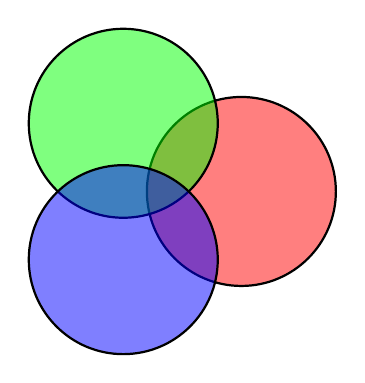
\begin{tikzpicture}[thick,fill opacity=0.5] 
  \filldraw[fill=red] (0:1cm) circle (12mm); 
  \filldraw[fill=green] (120:1cm) circle (12mm); 
  \filldraw[fill=blue] (-120:1cm) circle (12mm);
\end{tikzpicture}

\begin{tikzpicture}
  \draw [red](3cm,0cm) circle (4cm);
  \draw (0cm,0cm) circle (4cm);
  \draw [blue](-3cm,0cm) circle (4cm);
\end{tikzpicture}

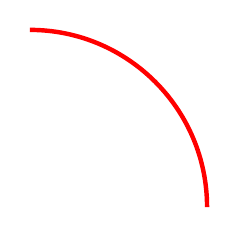
\begin{tikzpicture}[scale=0.25]
  \pgfmathsetmacro{\CircROne}{4.}
  \pgfmathsetmacro{\CircRTwo}{6.5}
  \pgfmathsetmacro{\CircRThree}{7.75}
  \pgfmathsetmacro{\CircRFour}{9.}
  \draw [ultra thick,red] (\CircRFour,0cm) arc (0:90:\CircRFour);
\end{tikzpicture}

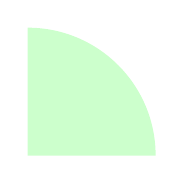
\begin{tikzpicture}[scale=0.25]
  \pgfmathsetmacro{\CircROne}{4.}
  \pgfmathsetmacro{\CircRTwo}{6.5}
  \pgfmathsetmacro{\CircRThree}{7.75}
  \pgfmathsetmacro{\CircRFour}{9.}
  % \draw [ultra thick,red] (\CircRFour,0cm) arc (0:90:\CircRFour);

  \fill[green!20!white] (0, 0) -- (\CircRTwo,0) arc (0:90:\CircRTwo) -- cycle;
\end{tikzpicture}

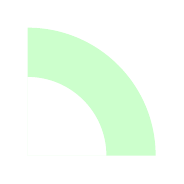
\begin{tikzpicture}[scale=0.25,even odd rule]]
  \pgfmathsetmacro{\CircROne}{4.}
  \pgfmathsetmacro{\CircRTwo}{6.5}
  \pgfmathsetmacro{\CircRThree}{7.75}
  \pgfmathsetmacro{\CircRFour}{9.}
  % \draw [ultra thick,red] (\CircRFour,0cm) arc (0:90:\CircRFour);

  \fill[fill=green!20!white] 
  (0, 0) -- (\CircRTwo,0) arc (0:90:\CircRTwo) -- cycle
  (0, 0) -- (\CircROne,0) arc (0:90:\CircROne) -- cycle;

\end{tikzpicture}

Another drawing

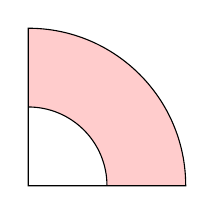
\begin{tikzpicture}[scale=1]]
  \filldraw[fill=red!20!white,even odd rule] 
  (0, 0) -- (2,0) arc (0:90:2) -- cycle
  (0, 0) -- (1,0) arc (0:90:1) -- cycle;
\end{tikzpicture}

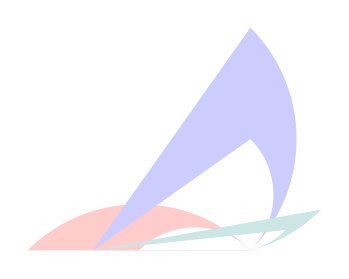
\begin{tikzpicture}[scale=1]]
  \fill[fill=red!20!white,even odd rule] 
  (0,0) -- (2,0) arc (45:135:2) -- cycle
  (0,0) -- (2,0) arc (45:135:1) -- cycle;

  \fill[fill=blue!20!white,even odd rule] 
  (0,0) -- (2,0) arc (-45:45:2) -- cycle
  (0,0) -- (2,0) arc (-45:45:1) -- cycle;

  \fill[fill=teal!20!white,even odd rule] 
  (0,0) -- (2,0) arc (-75:-45:2) -- cycle
  (0,0) -- (2,0) arc (-75:-45:1) -- cycle;
\end{tikzpicture}


Using double line

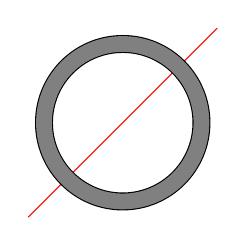
\begin{tikzpicture}
\draw[red] (-1.2,-1.2) -- (1.2,1.2);
\draw[double=gray, double distance=2mm] (0,0) circle (1);
\end{tikzpicture}


You should use a coordinate transformation for this, to get 
a proper starting point of the arc. Say, 
([shift=(t:r)] x, y) 
is the proper starting point, where (x,y) 
is the center and (t:r) is the polar coordinate of starting point

https://tex.stackexchange.com/questions/66216/draw-arc-in-tikz-when-center-of-circle-is-specified

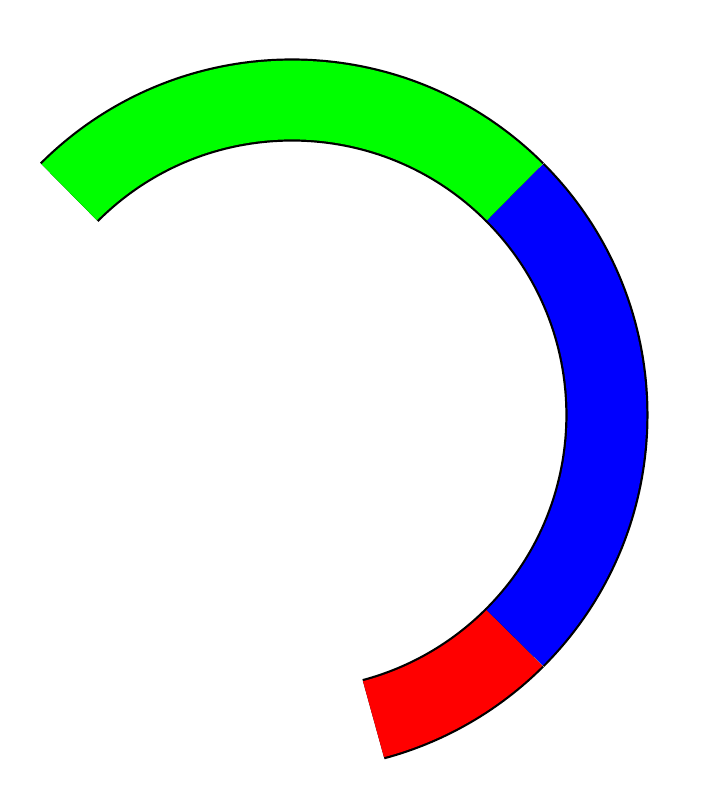
\begin{tikzpicture}
  \draw[thick,double=red, double distance=1cm] ([shift=(-75:4cm)] 4,0) arc (-75:-45:4);
  \draw[thick,double=blue, double distance=1cm] ([shift=(-45:4cm)] 4,0) arc (-45:45:4);
  \draw[thick,double=green, double distance=1cm] ([shift=(45:4cm)] 4,0) arc (45:135:4);
\end{tikzpicture}

\end{document}